\documentclass[11pt,letter]{article}
\usepackage{etex}
\usepackage[top=0.65in,bottom=0.9in,left=0.85in,right=0.85in]{geometry}

%\def\baselinestretch{1.25}
\def\baselinestretch{1.0}

\usepackage[greek, english]{babel}
%\usepackage{multicol}
\usepackage[thinlines]{easytable}

%\usepackage[draft]{graphicx}
\usepackage{graphicx}
\usepackage[export]{adjustbox}

\usepackage{caption}
\usepackage{subcaption}

\usepackage{setspace}
\usepackage{float}

% The use of the times package forces the use of the type-1 times
% roman font, but the times roman font does not look nice.
% Besides the times roman font still does not print correctly on
% the dopy printer.
%\usepackage{times}


\usepackage{fancyhdr}
\usepackage{amsmath}
\usepackage{amssymb}
\usepackage{bm}
\usepackage{bbold}
\usepackage{parskip}
\usepackage{url}

\newcommand{\kb}{\ensuremath{k_{\text{B}}}}

\newcommand{\bv}[1]{\ensuremath{\bm{#1}}}
\newcommand{\Lc}{\ensuremath{L_{\mathrm{c}}}}
\newcommand{\dsig}[1]{\ensuremath{ \frac{ d\,\sigma_{#1} }{d\,\Omega} }}

\newcommand{\isat}{\ensuremath{I_{\mathrm{sat}}}}
\newcommand{\iisat}{\ensuremath{I_{\mathrm{p}}/I_{\mathrm{sat}}}}
\newcommand{\Iqtof}{\ensuremath{I_{\bv{Q}\infty} }}
\newcommand{\Itof}[1]{\ensuremath{I_{\bv{#1}\infty} }}
\newcommand{\Iq}{\ensuremath{I_{\bv{Q}} }}
\newcommand{\iq}{\ensuremath{i_{\bv{Q}} }}
\newcommand{\Iqma}{\ensuremath{I_{\bv{Q}_{\text{MA}}} }}
\newcommand{\Ima}[1]{\ensuremath{I_{\bv{#1}_{\text{MA}}} }}
\newcommand{\iqma}{\ensuremath{i_{\bv{Q}_{\text{MA}}} }}
\newcommand{\jqma}{\ensuremath{j_{\bv{Q}_{\text{MA}}} }}
\newcommand{\Iqmatof}{\ensuremath{I_{\bv{Q}_{\text{MA}\infty}} }}
\newcommand{\is}{\ensuremath{i_{S}} }
\newcommand{\iqT}{\ensuremath{i_{\bv{Q}_{T}} }}
\newcommand{\ipith}{\ensuremath{i_{\bv{\pi}/\bv{\theta}}}}
\newcommand{\fpith}{\ensuremath{f_{\bv{\pi}/\bv{\theta}}}}
\newcommand{\iT}[1]{\ensuremath{i_{\bv{#1}_{T}} }}
\newcommand{\ima}[1]{\ensuremath{i_{\bv{#1}_{\text{MA}}} }}
\newcommand{\fma}[1]{\ensuremath{f_{\bv{#1}_{\text{MA}}} }}
\newcommand{\jma}[1]{\ensuremath{j_{\bv{#1}_{\text{MA}}} }}

\newcommand{\pin}{\ensuremath{ P_{\text{i}}} }
\newcommand{\pret}{\ensuremath{ P_{\text{r}}} }
\newcommand{\win}{\ensuremath{ w_{\text{in}}} }
\newcommand{\wret}{\ensuremath{ w_{\text{r}}} }
\newcommand{\wir}{\ensuremath{ w_{\text{IRS}}} }

\newcommand{\pgr}{\ensuremath{ P_{\text{gr}}} }
\newcommand{\wgr}{\ensuremath{ w_{\text{gr}}} }

\newcommand{\dbl}{\ensuremath{ \!\uparrow\! \downarrow \, }}
\newcommand{\spup}{\ensuremath{ \!\uparrow }}
\newcommand{\spdn}{\ensuremath{ \!\downarrow}}

\newcommand{\rdiag}{\ensuremath{ r_{\text{\tiny{111}}} } }
\newcommand{\awaist}{\ensuremath{ \alpha_{w} }}  
\newcommand{\awaistevap}{\ensuremath{ \alpha_{w,\text{evap}} }}  

\begin{document}

\section{ Estimation of systematic uncertainty in LDA due to trap parameters }  

To get an idea of the systematic uncertainty in the LDA temperature estimation
we will focus on the data point at $U_{0}/t_{0}=11.1$.  We make the following
three assumptions: 

\begin{enumerate} 

\item  \textbf{We have accurate knowledge of the atom number.} For the point at
$U_{0}/t_{0}=11.1$ it is $N=1.68\times 10^{5}$ atoms.

\item  \textbf{The central density of the sample is $1\leq n\leq 1.3$.}   It
turns out that if the atoms were to be all at $n<1$ then the temperature
necessary to reproduce our data would be very low, so we discard this scenario.
Experimentally we varied the atom number to obtain the largest Bragg scattering
signals,  we will use this as a guarantee that $n\geq 1$ at the center.   For
the assumed upper limit on $n$ we have the insitu images of the cloud, which
indicate that the central density is $n\simeq 1.1-1.2$, however there may be a
systematic uncertainty in the density measurement, so we extend the upper limit
to $n\leq1.3$ 

\item \textbf{The interaction strength is  $10.2 \leq U_{0}/t_{0} \leq 12.0$.}
The quantity that we calibrate more accurately in our trap is the lattice depth
at the center.  From the lattice modulation spectroscopic feature we have an
uncertainty in the lattice depth of $\pm3$\%.   The scattering length is known
accurately since the field is easily calibrated.  The field to scattering
length correspondance is well known\cite{Zurn2013}.  The $\pm3$\% error on the
lattice depth translates to $\pm8$\% on $U_{0}/t_{0}$, which corresponds to the
range given above.   

\end{enumerate}

The trap parameters that go into the LDA are: 
\begin{itemize}

\item Lattice depth, $v_{0}$ 

\item Compensation depth, $g_{0}$ 

\item Lattice waist, $w_{\mathrm{IR}}$ 

\item Compensation waist, $w_{\mathrm{GR}}$ 
\end{itemize}

In what follows we will vary each parameter independently, and also will vary
the depths and the waists together.   We will see how this affects the
temperature determination using the experimental data point at $U_{0}/t_{0}$
which has $S_{\bv{\pi}} = 1.96 \pm 0.12 $ 

\subsection{ Lattice depth} 

We vary the lattice depth $v_{0}$ from $v_{0}=6.8\,E_{r}$ to $v_{0}=7.2\,E_{r}$
and calculate the LDA for various temperatures.   For every point we adjust the
global chemical potential  so that the atom number is $N=1.68\times 10^{5}$ as
measured in the experiment.   The results are shown in Fig.~\ref{fig:01}.  We
will do similar variations for all the other parameters,  but will only include
a detailed explanation of the results in the caption of Fig.~\ref{fig:01}.  The
figures for the other parameters will follow the same logic.  

\begin{figure}[H]
    \centering 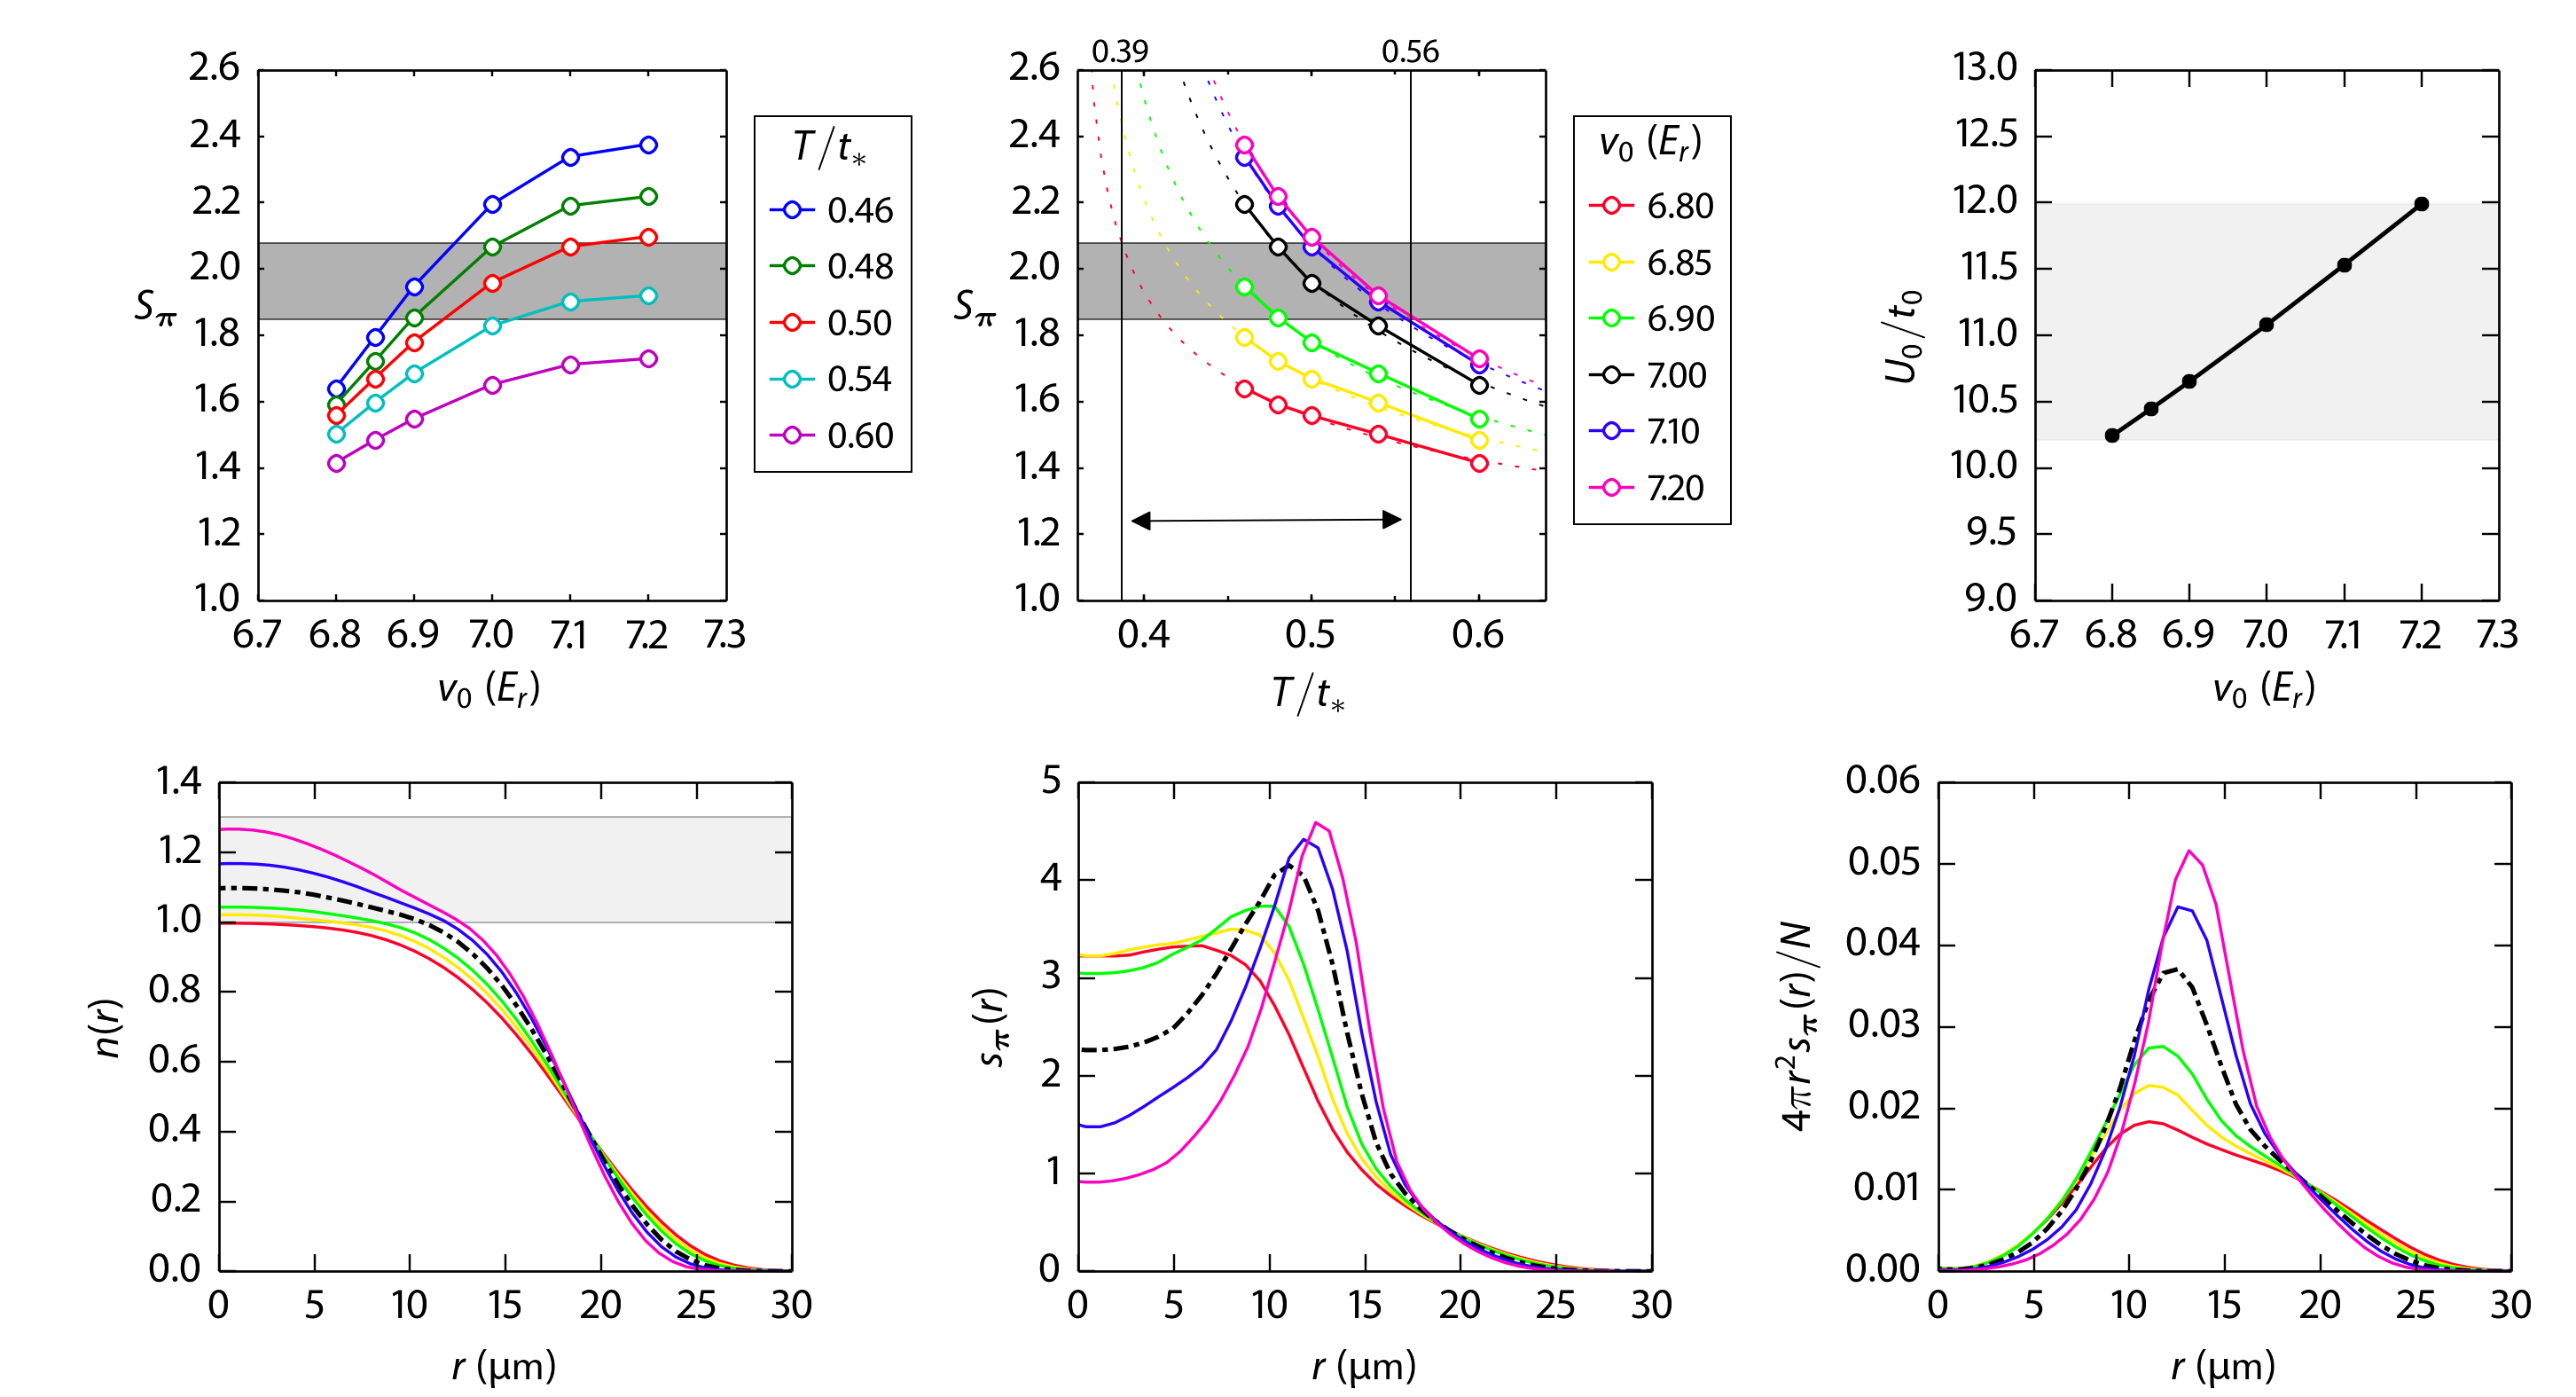
\includegraphics[width=\textwidth]{figures/01_LatticeDepth.png}
\caption{ The top left panel shows the variation of the trap averaged
$S_{\bv{\pi}}$ with lattice depth for various temperatures.   The shaded area
represents the experimental measurement.  The same data can be plotted as a
function of temperature for every value of $v_{0}$ as shown in the top central
panel.  The top central panel can be used to perform thermometry.  Notice that
we use the color black for the results at the nominal value of the varied
parameter (in this case $v_{0}=7\,E_{r}$).   The relevant range for the varied
parameter is obtained from conditions 2. and 3. in the list given at the
beginning of this document.   Condition 2 is represented in the bottom left
panel, which shows the density distribution.  If a value of the varied
parameter produces a central density outside the shaded area ($1\leq n
\leq1.3$), then it is not compatible with our experimental observations.
Similarly, condition 3 is represented in the top right panel.  If a value of
the varied parameter produces a value of $U_{0}/t_{0}$ outside the shaded area
then it is not consistent with our lattice depth calibration.   In this case,
condition 3 is the most restrictive and tells us that the relevant range for
$v_{0}$ is approximately $6.80\,E_{r} < v_{0} < 7.2\,E_{r}$.   We then go back
to the top central panel and for this range find what are the maximum and
minimum temperatures consistent with our measurement.   Since we cannot produce
LDA results at arbitrarily low $T/t_{*}$  we fit the available temperature data
to a third degree polynomial and extrapolate.   In this way we obtain a range
in $T/t_{*}$ that represents the systematic uncertainty of the parameter under
study.   A \textbf{major} caveat is that the third degree polynomial
extrapolation will most certainly \textbf{not} capture the divergent behaviour
of $S_{\bv{\pi}}$ as $T_{N}$ is approached. } 
\label{fig:01}
\end{figure}

\begin{figure}[H]
    \centering 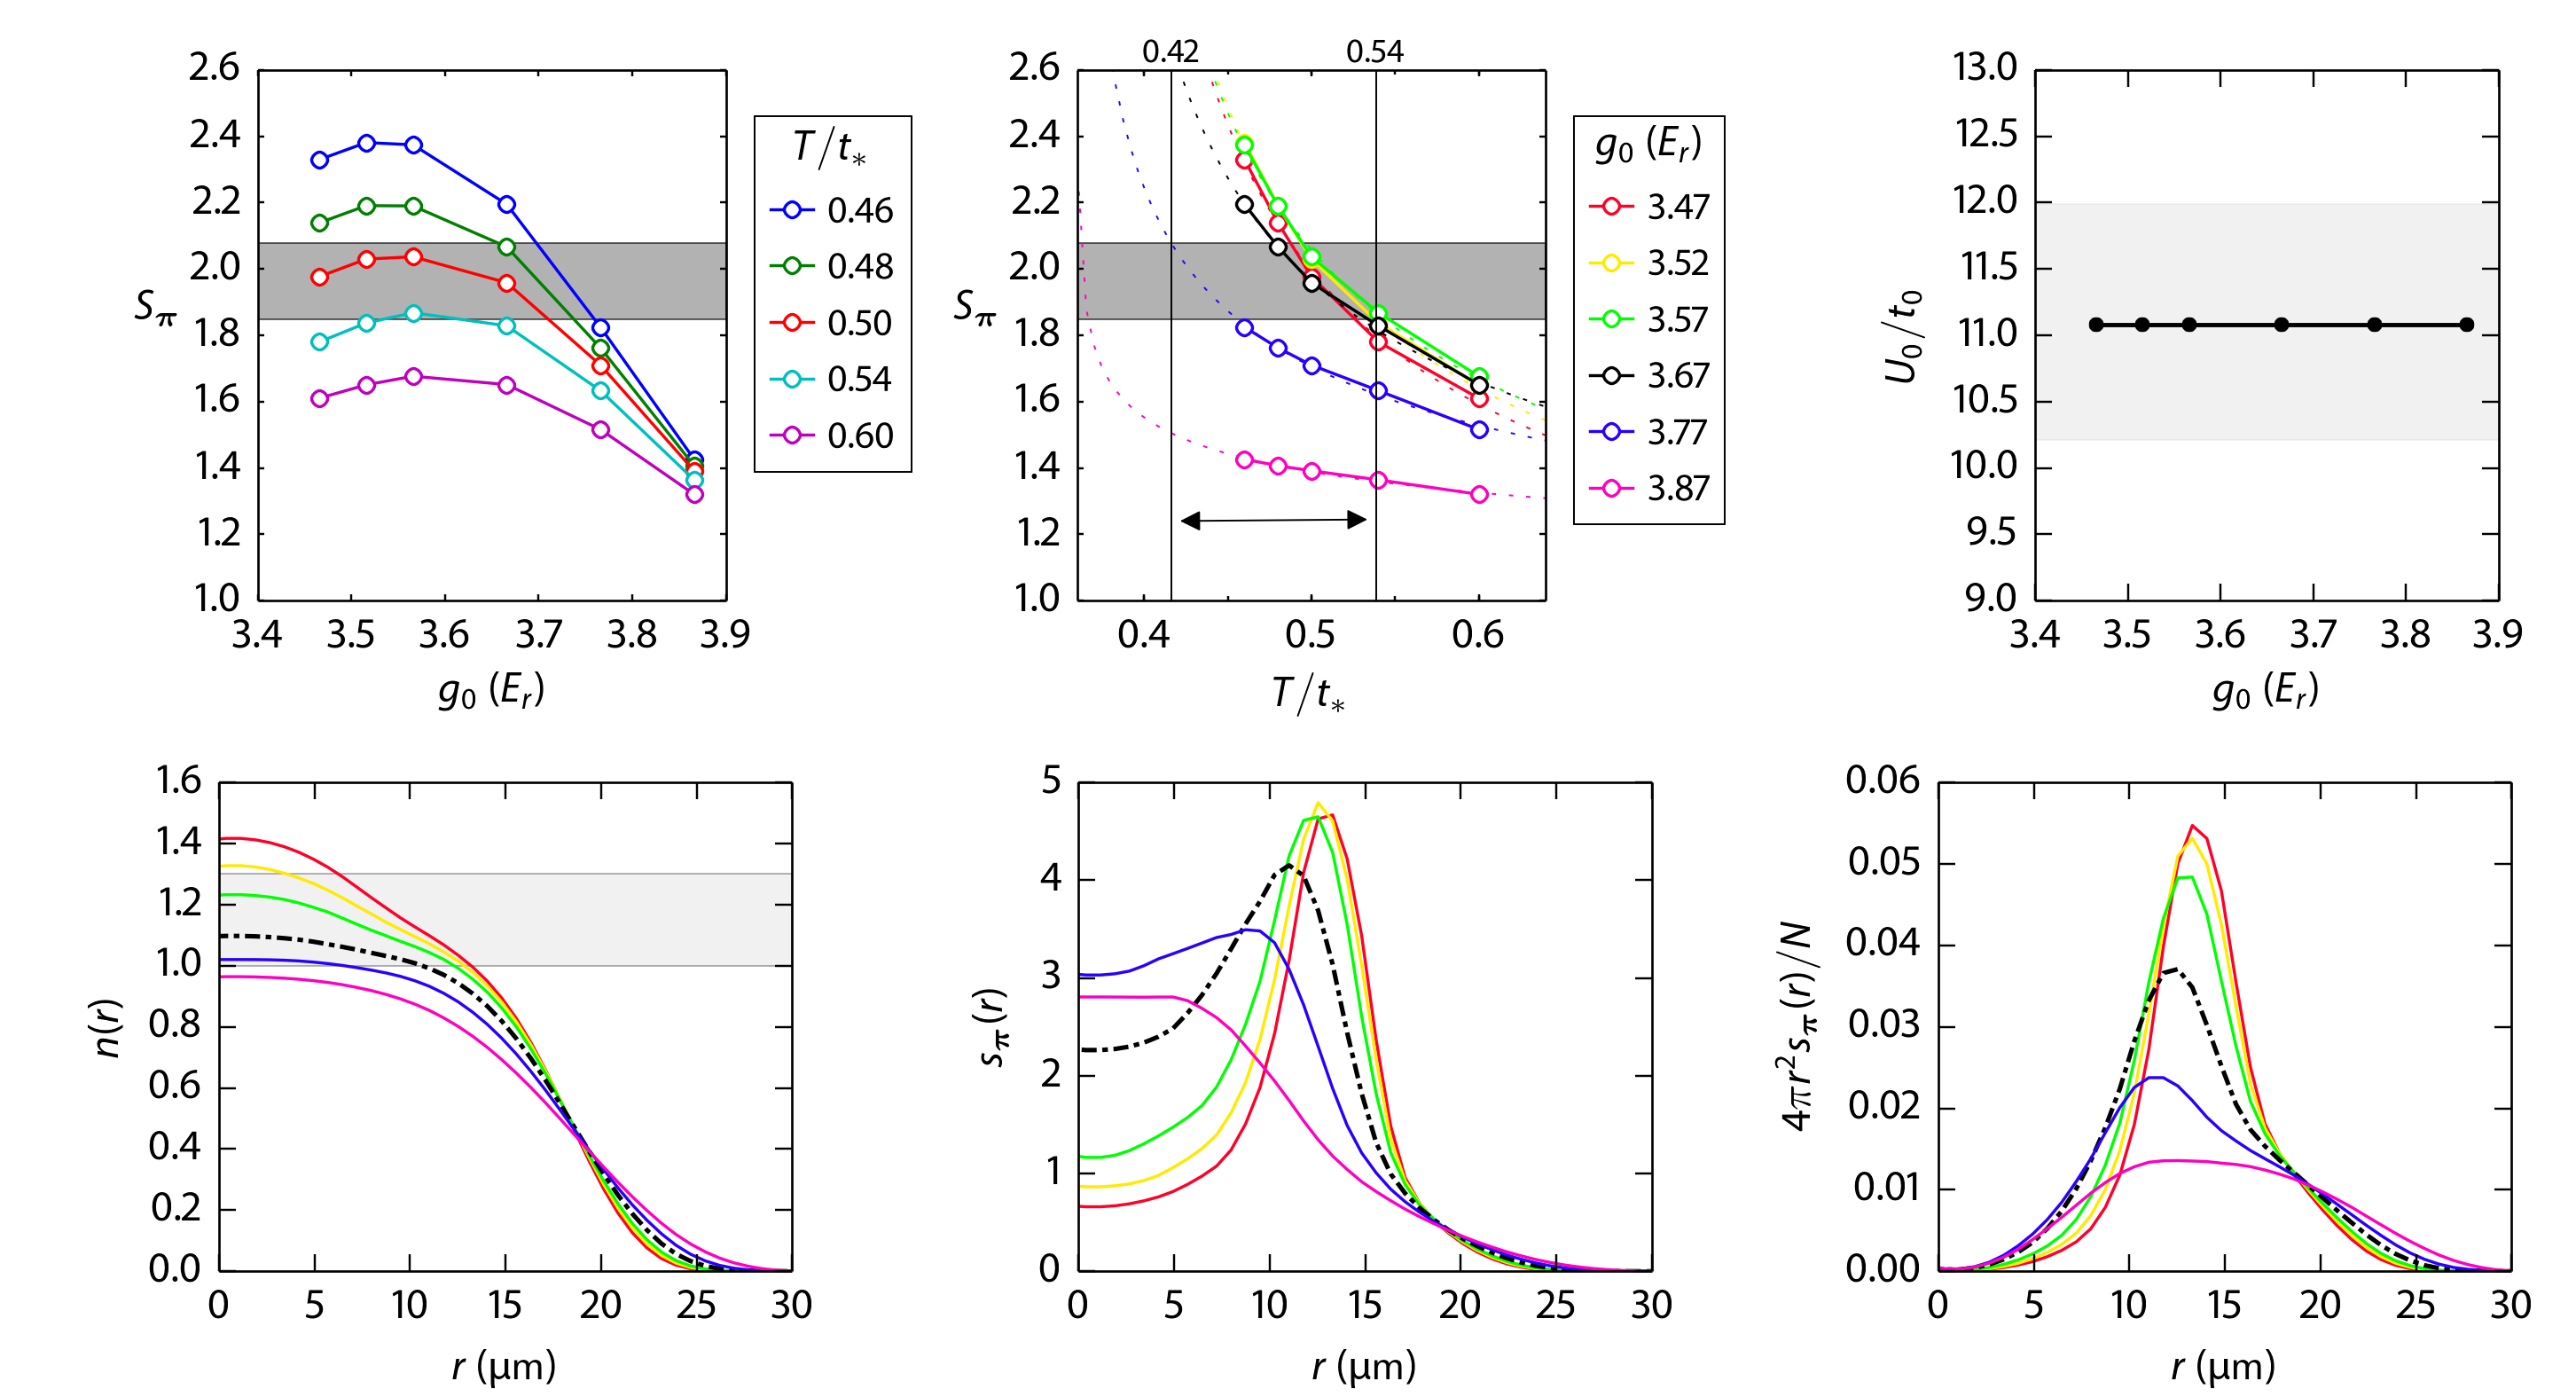
\includegraphics[width=\textwidth]{figures/02_CompDepth.png}
\caption{ }
\label{fig:02}
\end{figure}

\begin{figure}[H]
    \centering 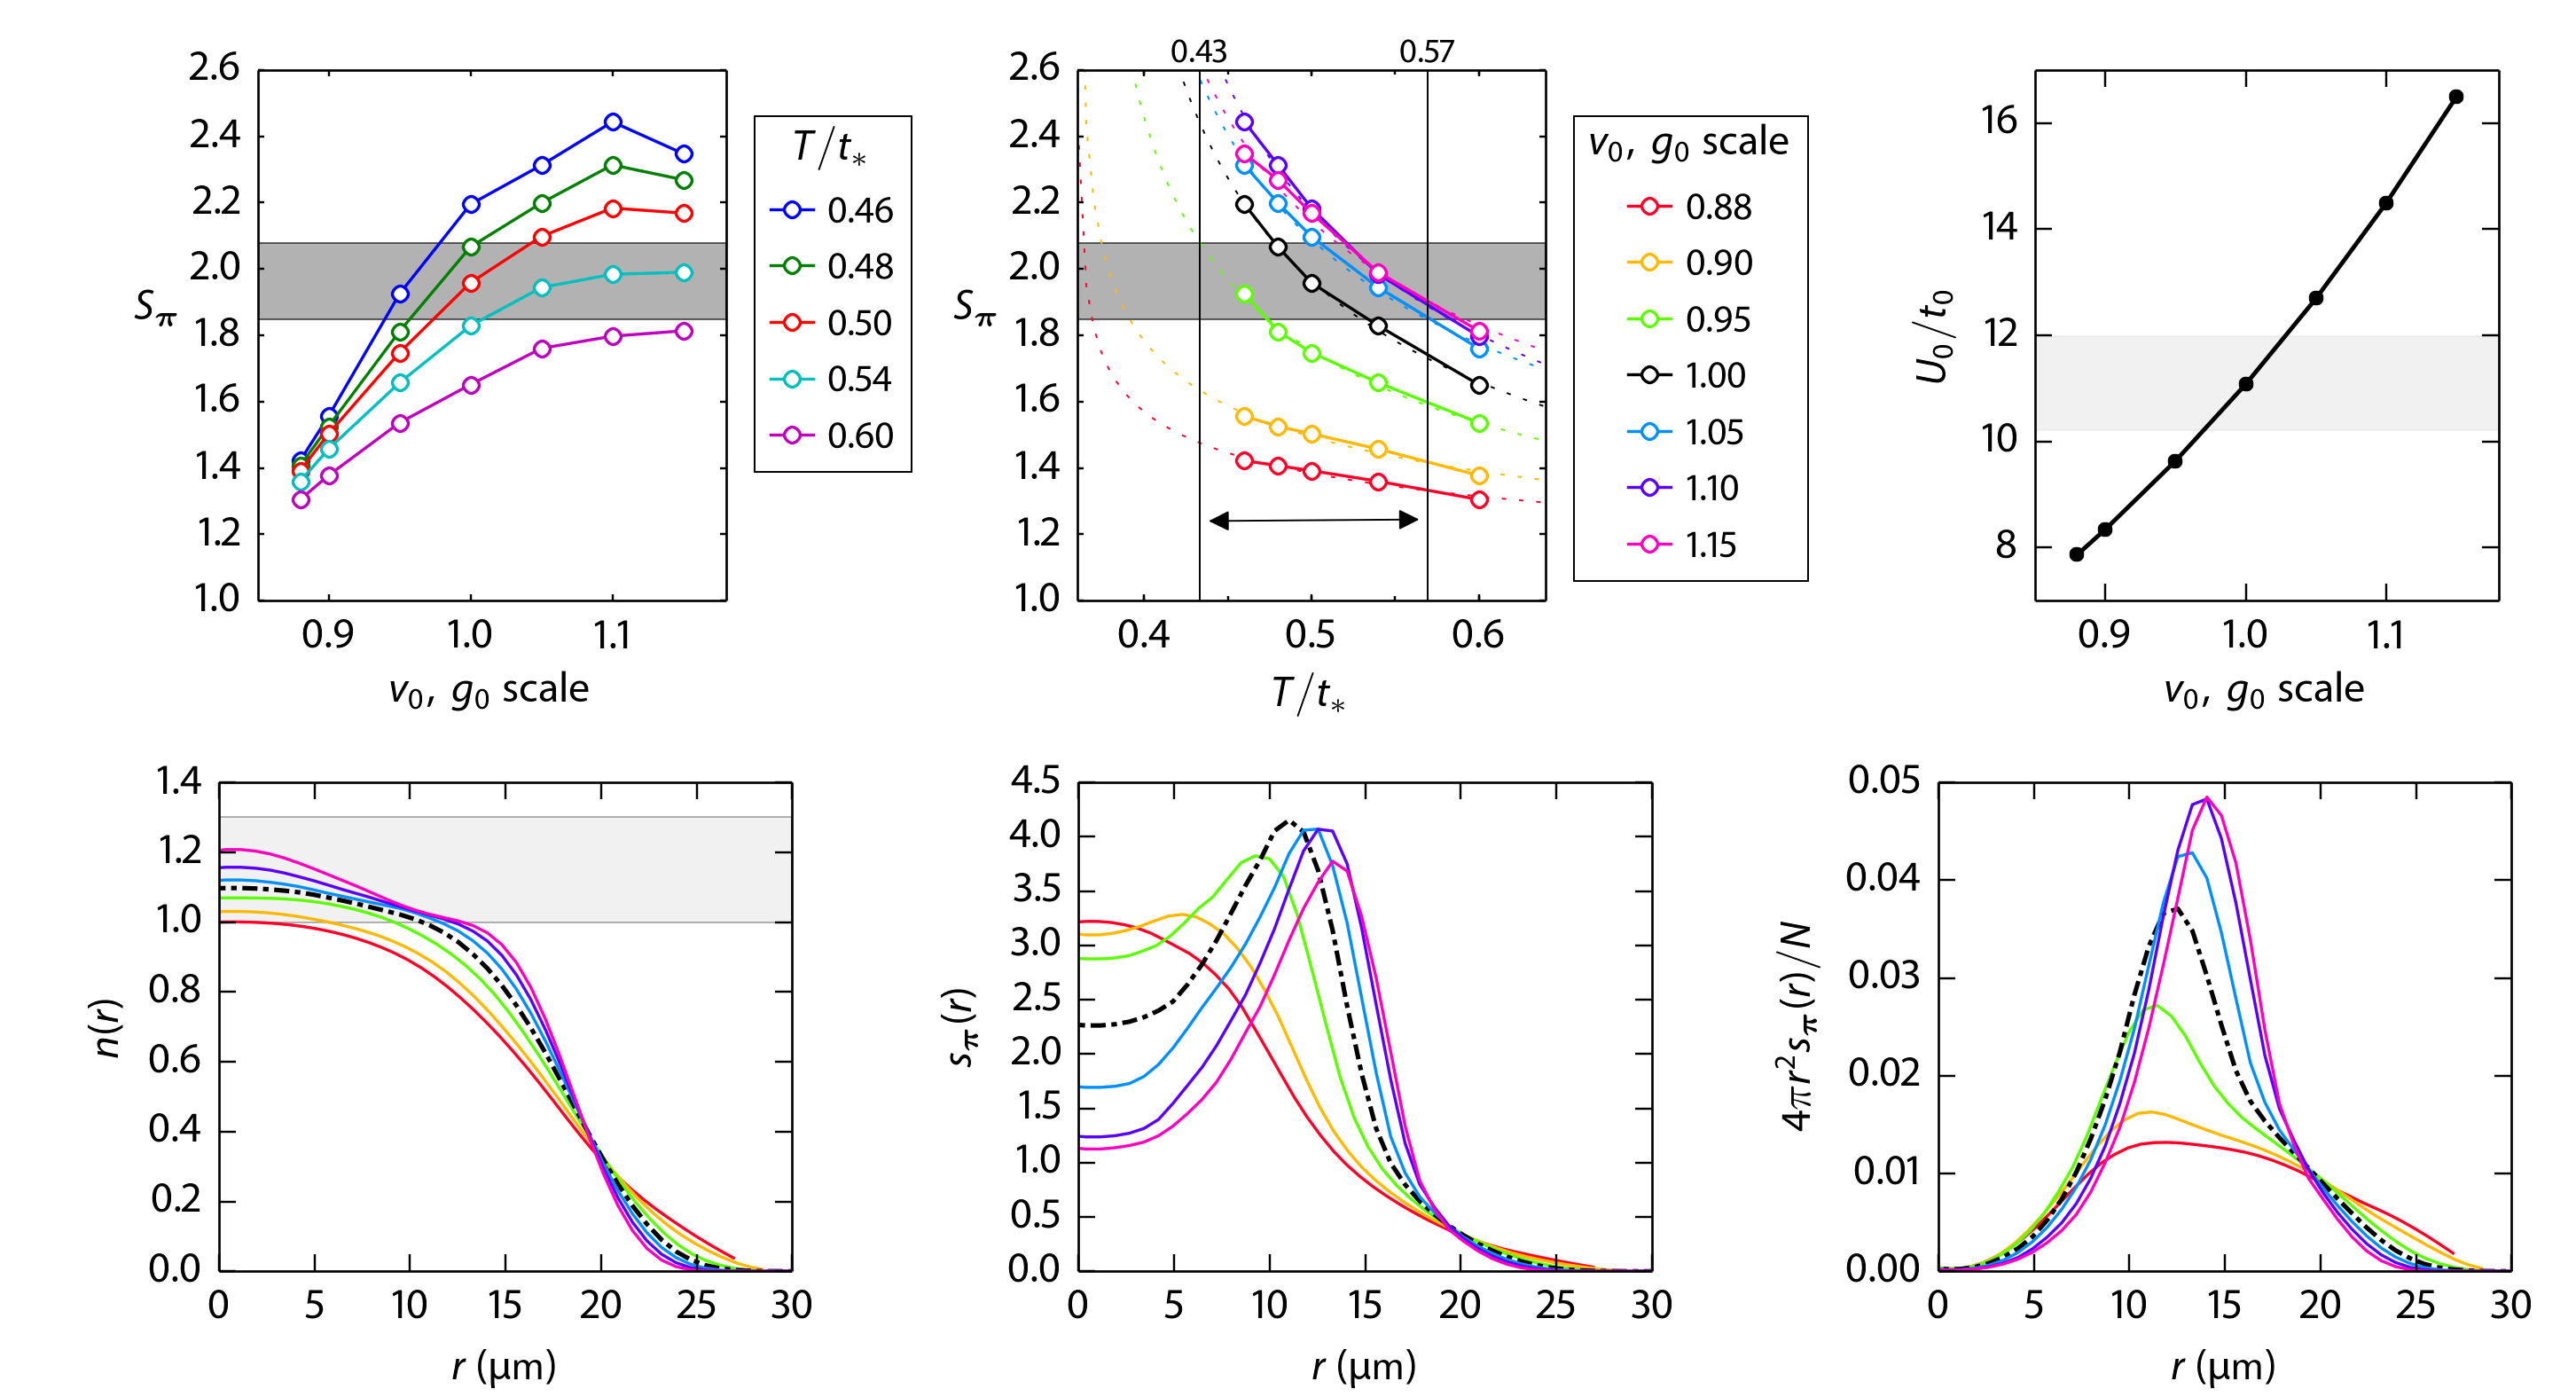
\includegraphics[width=\textwidth]{figures/03_Lattice+Comp.png}
\caption{ }
\label{fig:03}
\end{figure}

\begin{figure}[H]
    \centering 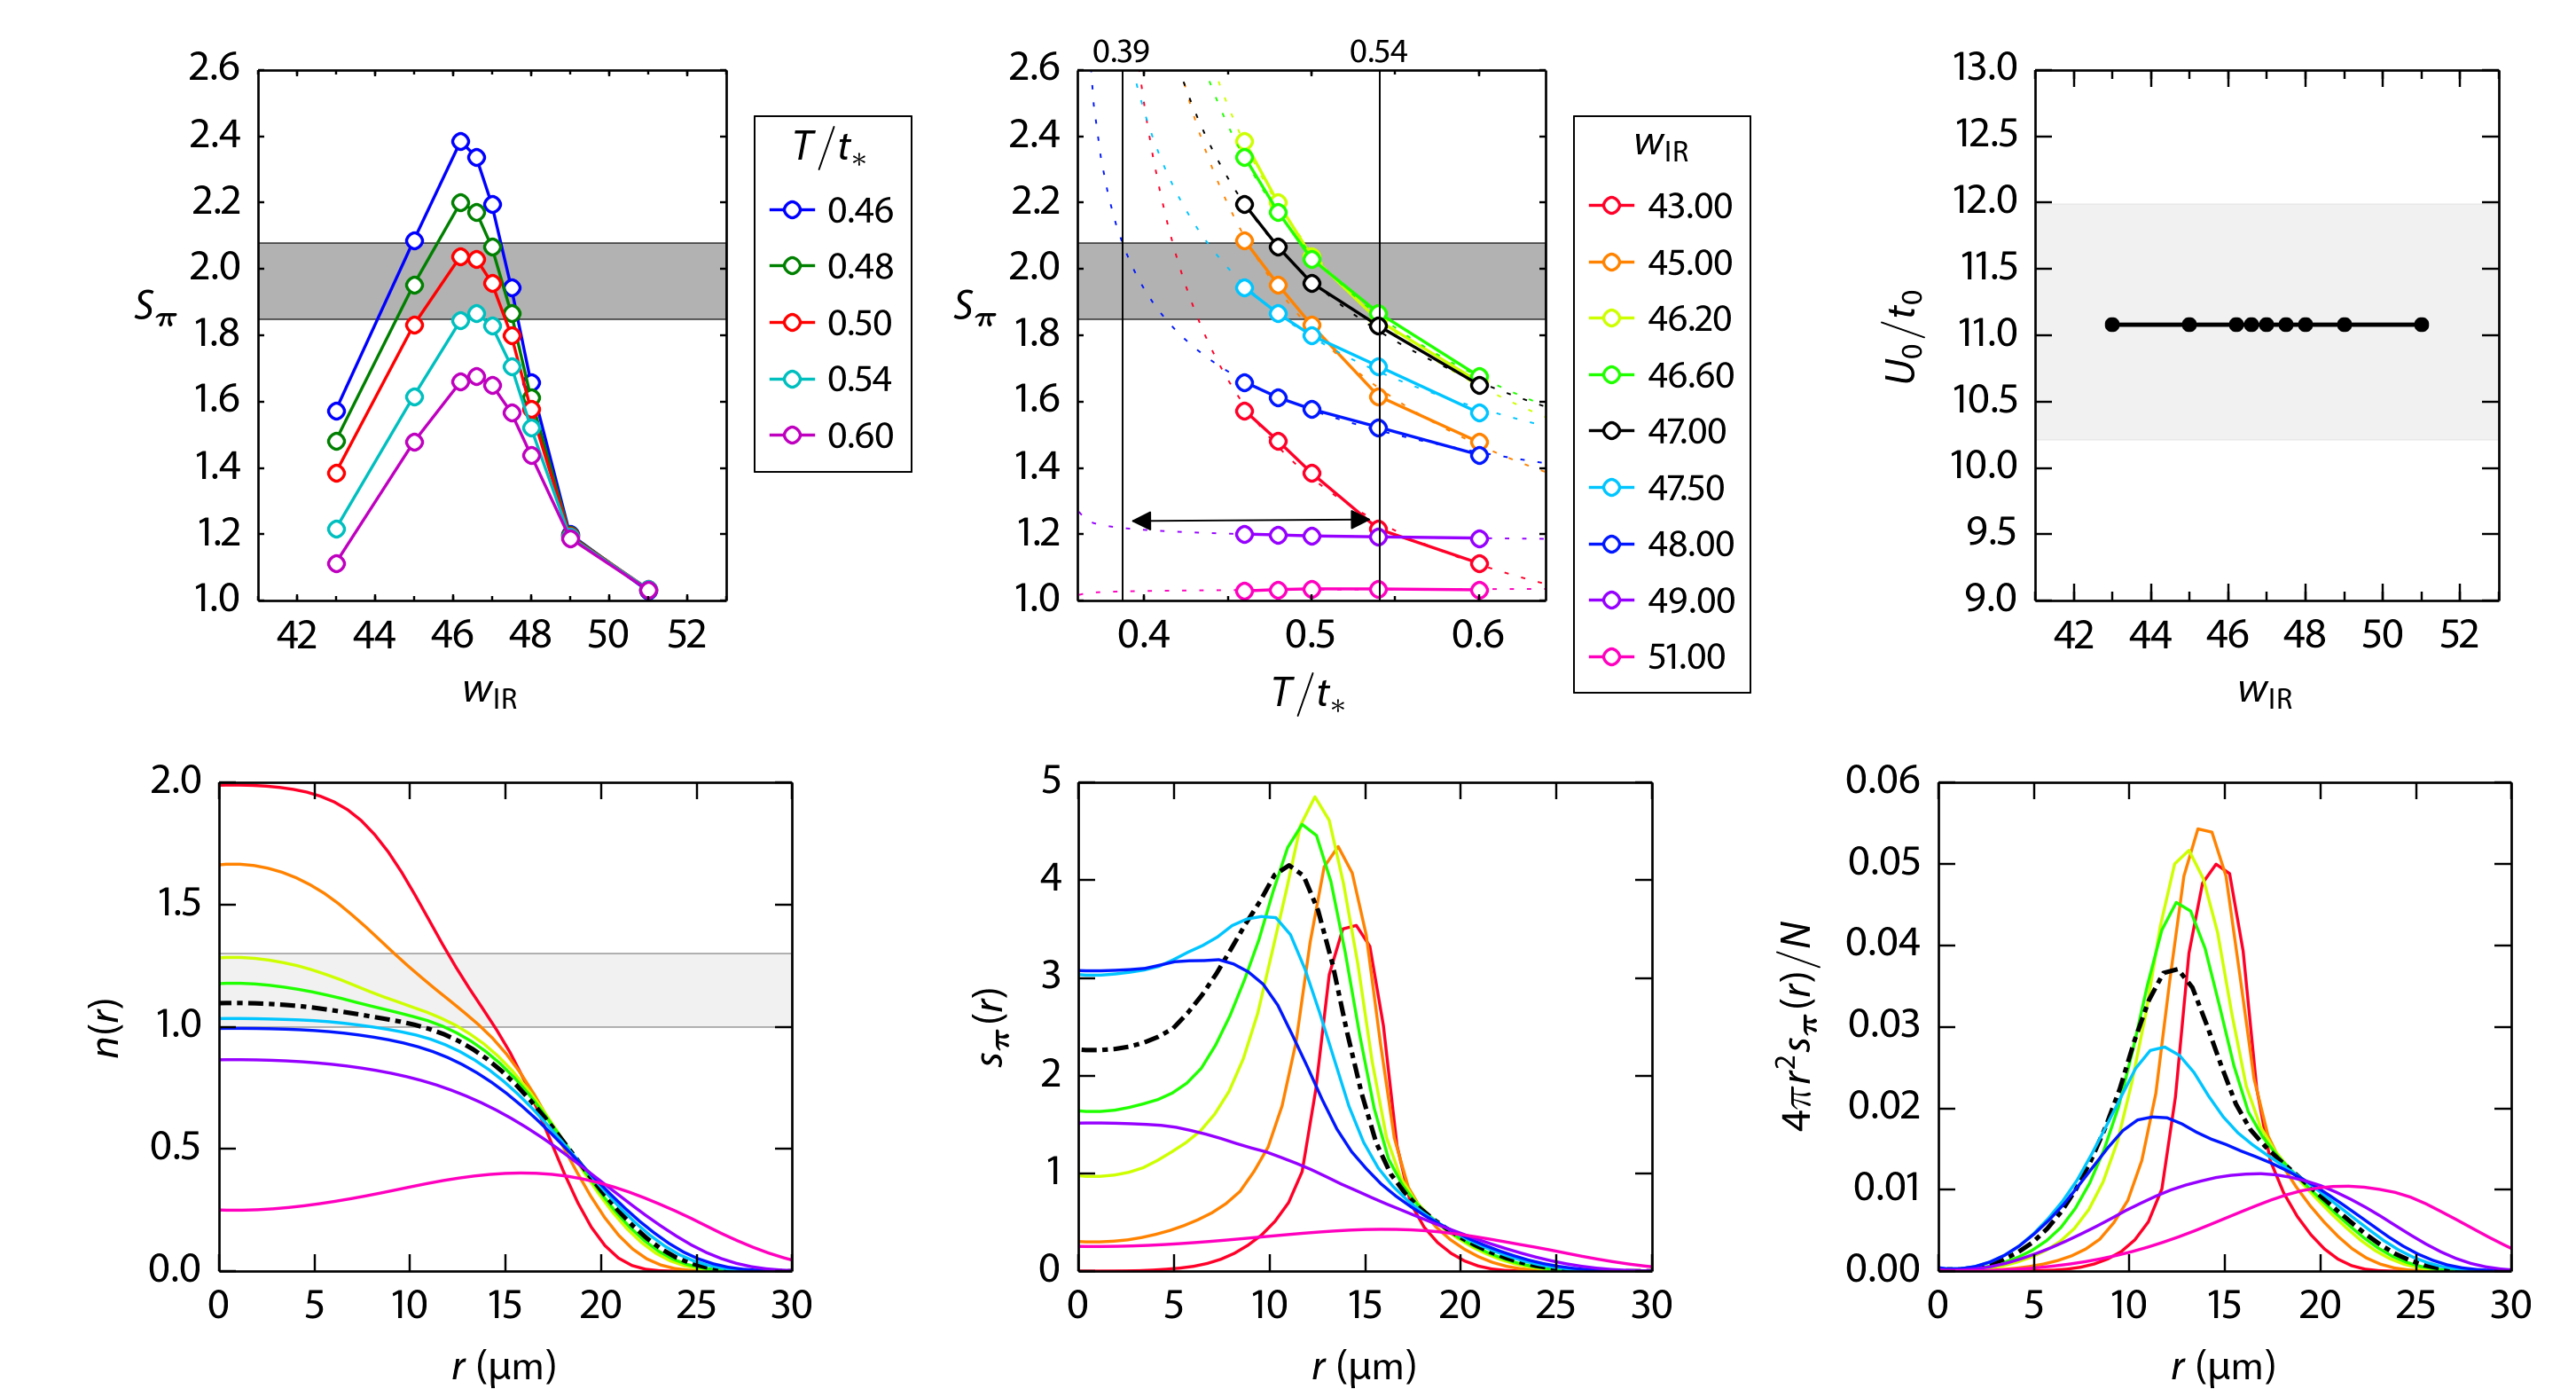
\includegraphics[width=\textwidth]{figures/04_wIR.png}
\caption{ }
\label{fig:04}
\end{figure}

\begin{figure}[H]
    \centering 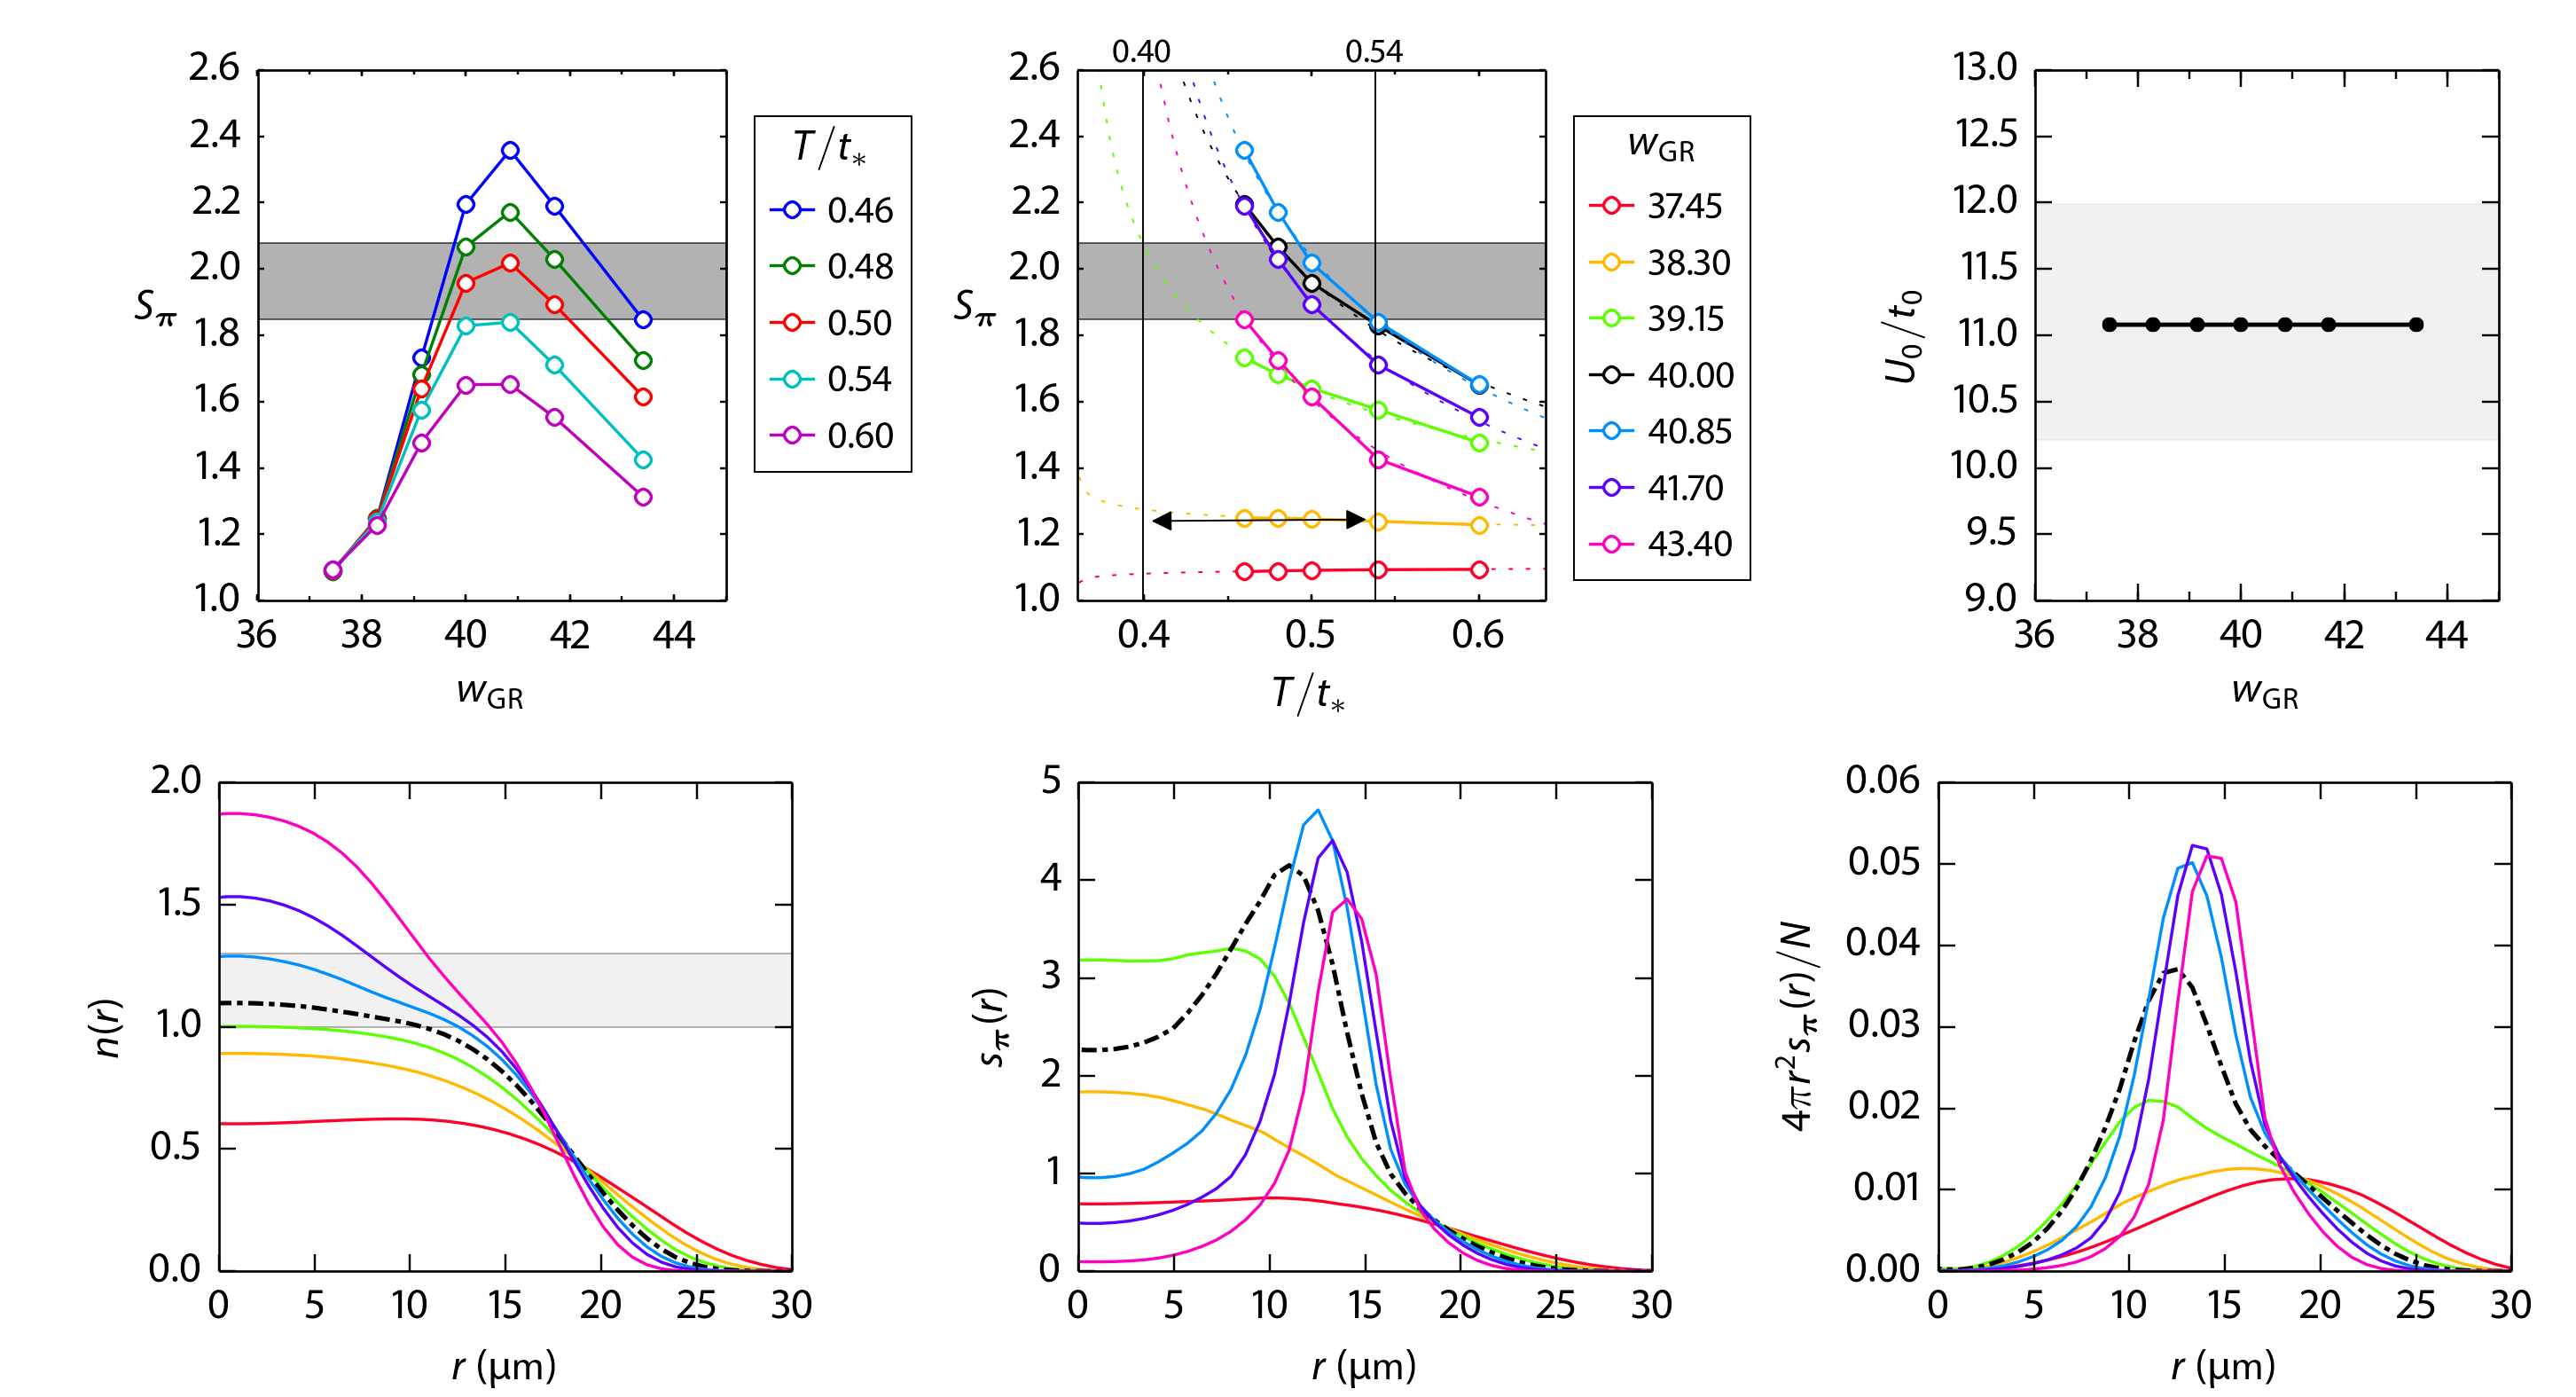
\includegraphics[width=\textwidth]{figures/05_wGR.png}
\caption{ }
\label{fig:05}
\end{figure}

\begin{figure}[H]
    \centering 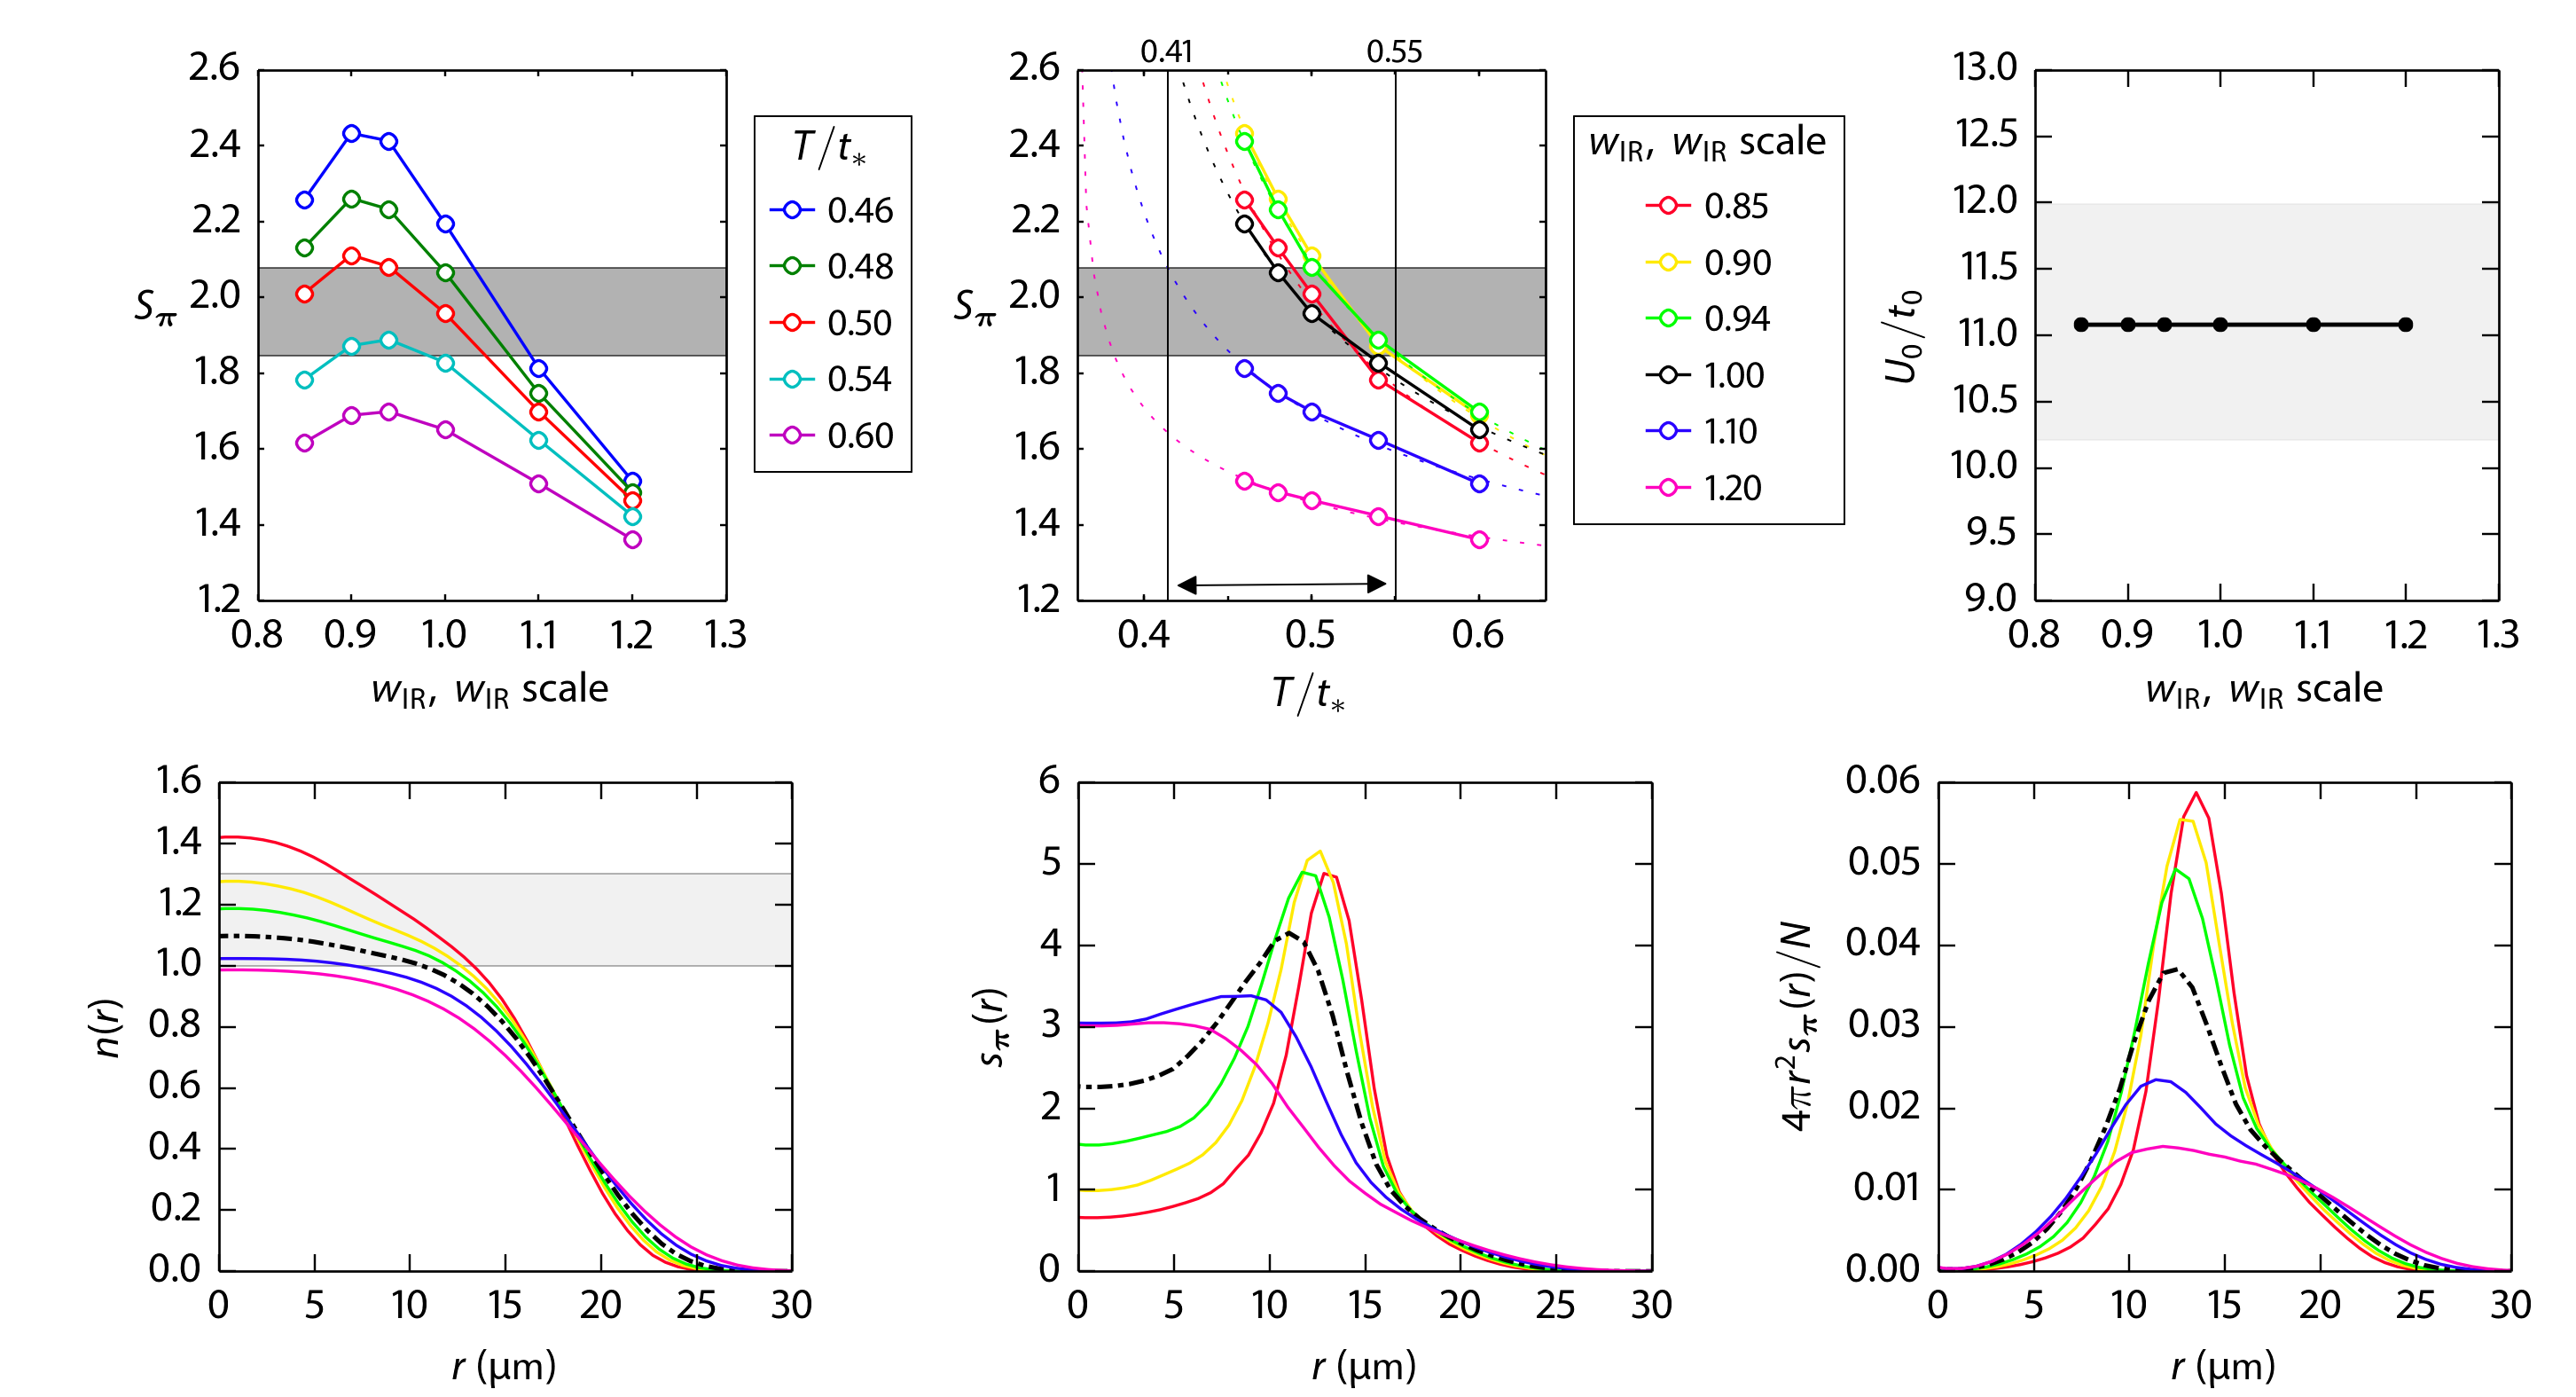
\includegraphics[width=\textwidth]{figures/06_wIR+wGR.png}
\caption{ }
\label{fig:06}
\end{figure}
 
\bibliographystyle{osa} 
\bibliography{writeup}

\end{document}




